\documentclass[11pt]{article}
\usepackage{fullpage,amsmath,amsfonts,mathpazo,microtype,nicefrac,graphicx,verbatimbox,hyperref,listings,enumitem,amssymb,float,fancyhdr}
\hypersetup{
  colorlinks = true,
  allcolors = {cyan}
}

\title{
\vspace{1cm}
\textmd{\textbf{AM205 Final Project: Modulo-n Lights Out}}\\
}

\author{\textbf{Shawn Pan and Andrew Ross}}
\date{\today}

%----------------------------------------------------------------------------------------

\begin{document}

\maketitle

\section*{Introduction}

\paragraph{} Lights Out is an electronic puzzle game released by Tiger Electronics (who notably also developed the \href{https://en.wikipedia.org/wiki/Furby}{Furby}) in 1995. An individual puzzle in Lights Out consists of a configuration of lit and unlit buttons on a 5x5 grid. Pressing any button toggles its state and that of the four adjacent buttons, and the goal is to turn all lights off in as few moves as possible.

\paragraph{} The effect of any sequence of presses can be represented as a modulo 2 sum of vectors (where each 2D board coordinate is mapped to a 1D vector position), and because summation is commutative, the sequence of presses will have the same effect regardless of its order. We can represent the constraints of the problem as a system of equations in $\mathbb{Z}_2$ (i.e. modular arithmetic on $\{0, 1\}$), which we can more helpfully write as a matrix equation

\begin{equation}
\text{mod}_2(Ax) = b,
\end{equation}

\noindent where $b = \langle g_{11}, g_{12}, \cdots, g_{15}, g_{21}, \cdots, g_{55} \rangle$ is the length-25 vector of grid states $g_{ij}$, which are 1 if lit and 0 otherwise, $x$ is the length-25 vector of presses, and $A$ is a matrix that encodes the transitions, which looks like
\begin{equation}
  A = \left (
  \setlength{\tabcolsep}{2pt}
  {\tiny %
  \begin{tabular}{ccccccccccccccccccccccccc}
1 & 1 & 0 & 0 & 0 & 1 & 0 & 0 & 0 & 0 & 0 & 0 & 0 & 0 & 0 & 0 & 0 & 0 & 0 & 0 & 0 & 0 & 0 & 0 & 0\\
1 & 1 & 1 & 0 & 0 & 0 & 1 & 0 & 0 & 0 & 0 & 0 & 0 & 0 & 0 & 0 & 0 & 0 & 0 & 0 & 0 & 0 & 0 & 0 & 0\\
0 & 1 & 1 & 1 & 0 & 0 & 0 & 1 & 0 & 0 & 0 & 0 & 0 & 0 & 0 & 0 & 0 & 0 & 0 & 0 & 0 & 0 & 0 & 0 & 0\\
0 & 0 & 1 & 1 & 1 & 0 & 0 & 0 & 1 & 0 & 0 & 0 & 0 & 0 & 0 & 0 & 0 & 0 & 0 & 0 & 0 & 0 & 0 & 0 & 0\\
0 & 0 & 0 & 1 & 1 & 0 & 0 & 0 & 0 & 1 & 0 & 0 & 0 & 0 & 0 & 0 & 0 & 0 & 0 & 0 & 0 & 0 & 0 & 0 & 0\\
1 & 0 & 0 & 0 & 0 & 1 & 1 & 0 & 0 & 0 & 1 & 0 & 0 & 0 & 0 & 0 & 0 & 0 & 0 & 0 & 0 & 0 & 0 & 0 & 0\\
0 & 1 & 0 & 0 & 0 & 1 & 1 & 1 & 0 & 0 & 0 & 1 & 0 & 0 & 0 & 0 & 0 & 0 & 0 & 0 & 0 & 0 & 0 & 0 & 0\\
0 & 0 & 1 & 0 & 0 & 0 & 1 & 1 & 1 & 0 & 0 & 0 & 1 & 0 & 0 & 0 & 0 & 0 & 0 & 0 & 0 & 0 & 0 & 0 & 0\\
0 & 0 & 0 & 1 & 0 & 0 & 0 & 1 & 1 & 1 & 0 & 0 & 0 & 1 & 0 & 0 & 0 & 0 & 0 & 0 & 0 & 0 & 0 & 0 & 0\\
0 & 0 & 0 & 0 & 1 & 0 & 0 & 0 & 1 & 1 & 0 & 0 & 0 & 0 & 1 & 0 & 0 & 0 & 0 & 0 & 0 & 0 & 0 & 0 & 0\\
0 & 0 & 0 & 0 & 0 & 1 & 0 & 0 & 0 & 0 & 1 & 1 & 0 & 0 & 0 & 1 & 0 & 0 & 0 & 0 & 0 & 0 & 0 & 0 & 0\\
0 & 0 & 0 & 0 & 0 & 0 & 1 & 0 & 0 & 0 & 1 & 1 & 1 & 0 & 0 & 0 & 1 & 0 & 0 & 0 & 0 & 0 & 0 & 0 & 0\\
0 & 0 & 0 & 0 & 0 & 0 & 0 & 1 & 0 & 0 & 0 & 1 & 1 & 1 & 0 & 0 & 0 & 1 & 0 & 0 & 0 & 0 & 0 & 0 & 0\\
0 & 0 & 0 & 0 & 0 & 0 & 0 & 0 & 1 & 0 & 0 & 0 & 1 & 1 & 1 & 0 & 0 & 0 & 1 & 0 & 0 & 0 & 0 & 0 & 0\\
0 & 0 & 0 & 0 & 0 & 0 & 0 & 0 & 0 & 1 & 0 & 0 & 0 & 1 & 1 & 0 & 0 & 0 & 0 & 1 & 0 & 0 & 0 & 0 & 0\\
0 & 0 & 0 & 0 & 0 & 0 & 0 & 0 & 0 & 0 & 1 & 0 & 0 & 0 & 0 & 1 & 1 & 0 & 0 & 0 & 1 & 0 & 0 & 0 & 0\\
0 & 0 & 0 & 0 & 0 & 0 & 0 & 0 & 0 & 0 & 0 & 1 & 0 & 0 & 0 & 1 & 1 & 1 & 0 & 0 & 0 & 1 & 0 & 0 & 0\\
0 & 0 & 0 & 0 & 0 & 0 & 0 & 0 & 0 & 0 & 0 & 0 & 1 & 0 & 0 & 0 & 1 & 1 & 1 & 0 & 0 & 0 & 1 & 0 & 0\\
0 & 0 & 0 & 0 & 0 & 0 & 0 & 0 & 0 & 0 & 0 & 0 & 0 & 1 & 0 & 0 & 0 & 1 & 1 & 1 & 0 & 0 & 0 & 1 & 0\\
0 & 0 & 0 & 0 & 0 & 0 & 0 & 0 & 0 & 0 & 0 & 0 & 0 & 0 & 1 & 0 & 0 & 0 & 1 & 1 & 0 & 0 & 0 & 0 & 1\\
0 & 0 & 0 & 0 & 0 & 0 & 0 & 0 & 0 & 0 & 0 & 0 & 0 & 0 & 0 & 1 & 0 & 0 & 0 & 0 & 1 & 1 & 0 & 0 & 0\\
0 & 0 & 0 & 0 & 0 & 0 & 0 & 0 & 0 & 0 & 0 & 0 & 0 & 0 & 0 & 0 & 1 & 0 & 0 & 0 & 1 & 1 & 1 & 0 & 0\\
0 & 0 & 0 & 0 & 0 & 0 & 0 & 0 & 0 & 0 & 0 & 0 & 0 & 0 & 0 & 0 & 0 & 1 & 0 & 0 & 0 & 1 & 1 & 1 & 0\\
0 & 0 & 0 & 0 & 0 & 0 & 0 & 0 & 0 & 0 & 0 & 0 & 0 & 0 & 0 & 0 & 0 & 0 & 1 & 0 & 0 & 0 & 1 & 1 & 1\\
0 & 0 & 0 & 0 & 0 & 0 & 0 & 0 & 0 & 0 & 0 & 0 & 0 & 0 & 0 & 0 & 0 & 0 & 0 & 1 & 0 & 0 & 0 & 1 & 1
    \end{tabular}
  }
  \right ).
  \label{a}
\end{equation}

\paragraph{} There are many ways to solve this matrix equation; in the case that $A$ is invertible, we can find its inverse $A^{-1}$ and obtain a unique solution $x = A^{-1}b$. Alternatively, we can use a factorization technique such as the LU decomposition to find $x$ more efficiently. In the case that $A$ isn't invertible, then in general it is possible that there may not be any $x$ such that $Ax = b$, and if there is, then $x$ will no longer be unique (although the shortest $x$, i.e. the $x$ that minimizes $\sum x_i$, may still be).

\subsection*{Previous Work}

\paragraph{} \cite{jaap} provides a great analysis of the core mathematics of the game and devotes a significant amount of time to generalizing board dimensions, with some limited discussion of generalizing number of button states. \cite{giffen} and \cite{involve} do a significant amount of work generalizing it to arbitrary transition matrices along with an arbitrary number of states by framing it as a graph coloring problem. One problem that \cite{jaap}, \cite{giffen}, and \cite{involve} all focus on is that of determining always-winnability for a given transition matrix $A$, initial grid state $b$, and modular domain $\mathbb{Z}_k$ -- and the dimensionality of the nullspace when it doesn't hold.

\subsection*{Our Contributions}

\paragraph{} We demonstrate a software package we wrote to solve Lights Out puzzles in $\mathbb{Z}_k$ with arbitrary and even singular (when possible) transition matrices, along with video visualizations of the intermediate states. We reproduce and generalize results tables from \cite{jaap} and confirm that they agree with theorems proved in \cite{giffen} and \cite{involve}.

\paragraph{} Solutions to light puzzles (arrays of press patterns) can also be interepreted as grids. We consider the recursive problem of solving a grid, then solving its solution, and so on, until we reach a state we have already seen or one that cannot be solved. The simplest version of this (a complete cycle of length 1) corresponds exactly to eigenvectors of the transition matrix with eigenvalue 1. We present our results and attempt to relate them to the theoretical work in \cite{jaap}, \cite{giffen}, and \cite{involve}.

\section*{Solvability and Quiet Patterns}

\paragraph{} \cite{jaap} presents tables of results for the transition matrix \eqref{a} at various dimensions in $\mathbb{Z}_2$ and $\mathbb{Z}_3$. In Figure \ref{nullity}, we reproduce them (up to 15x15) for $\mathbb{Z}_2$ to $\mathbb{Z}_{15}$.

\begin{figure}
\caption{Plots of the dimension of the nullspace of the standard Lights Out transition matrix at various grid sizes and moduli}
\label{nullity}
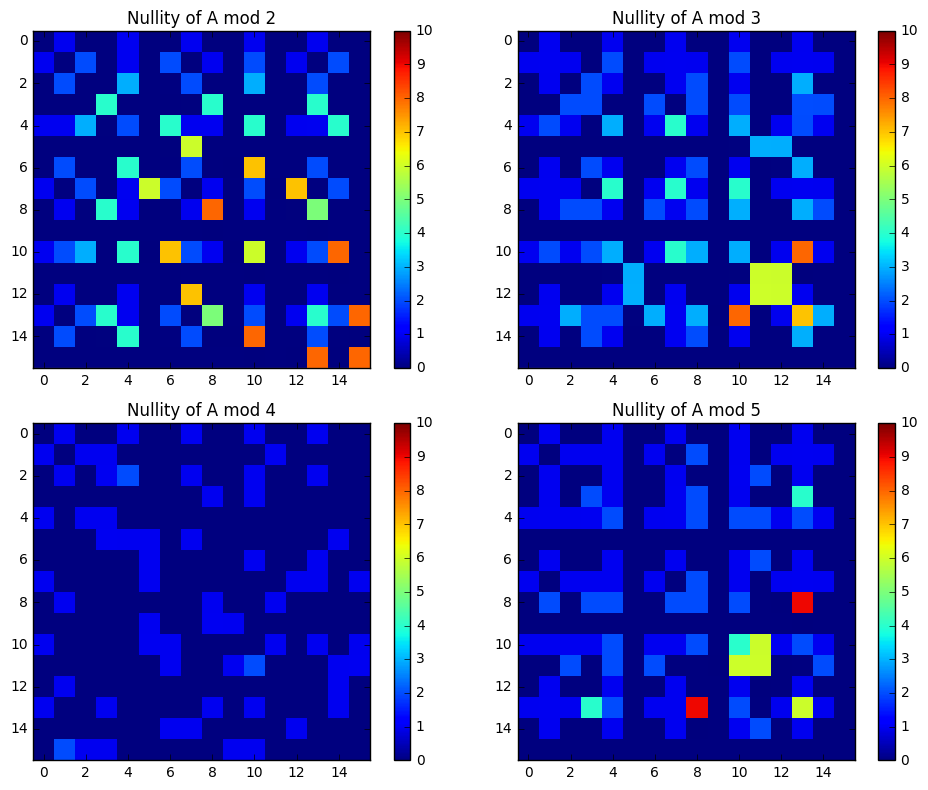
\includegraphics[width=\textwidth]{nullity.png}
\end{figure}

\begin{figure}
\caption{Plots of whether $\text{gcd}(\det(A(m,n)), k) = 1$ for $k,m,n \in \{2,3,...,15\}$}
\label{relprime}
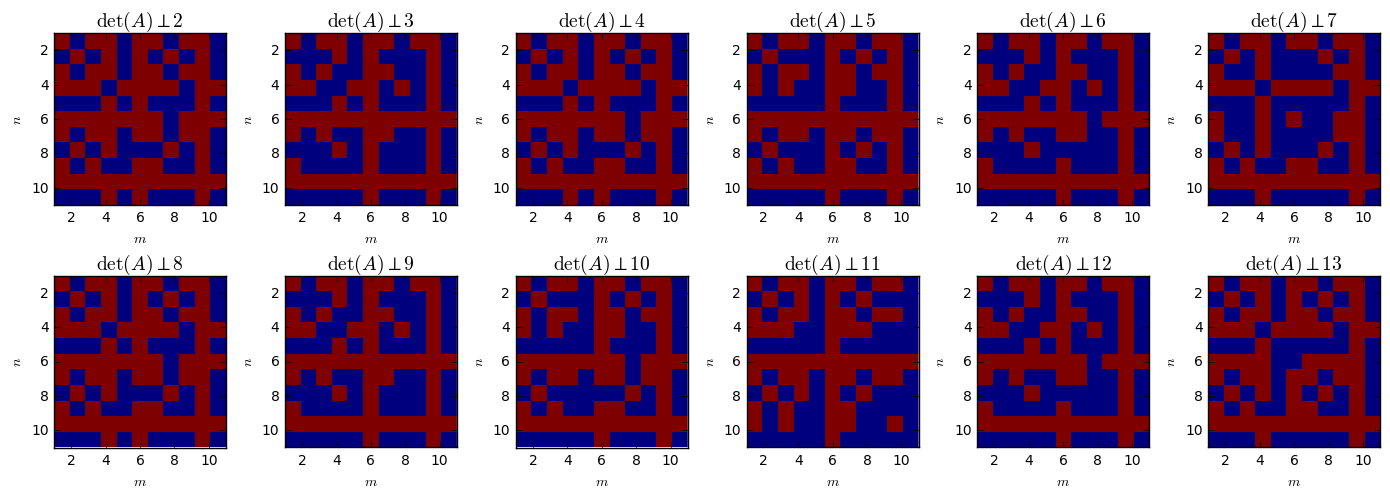
\includegraphics[width=\textwidth]{relprime.png}
\end{figure}

\paragraph{} Although we generated those results by finding the LU factorization of $A$ at each dimension and modularity, one result from \cite{involve} is that, for solvability to hold for a transition matrix $A$ at any modularity $k$, $\det(A)$ (computed without any modular operations) must be relatively prime to $k$, i.e. $\text{gcd}(\det(A), k) = 1$. We demonstrate this in Figure \ref{relprime} (which can be visually checked against Figure \ref{nullity}).

\clearpage

\begin{thebibliography}{9}
\bibitem{jaap}
  J. Scherphuis, \textit{The Mathematics of Lights Out},
  \href{http://www.jaapsch.net/puzzles/lomath.htm}{http://www.jaapsch.net/puzzles/lomath.htm}.
  Accessed December 2016.
\bibitem{giffen}
  A. Giffen and D. B. Parker, \textit{On Generalizing the "Lights Out" Game and a Generalization of Parity Domination}, preprint, 2009. Available at \href{http://faculty.gvsu.edu/parkerda/profstuff/papers/hyperlogpd.pdf}{http://faculty.gvsu.edu/parkerda/profstuff/papers/hyperlogpd.pdflink}.
\bibitem{involve}
  S. Edwards, V. Elandt, N. James, K. Johnson, Z. Mitchell, and D. Stephenson, \textit{Lights Out on finite graphs}, Involve 3 (2010), 17-32. Available at \href{http://msp.org/involve/2010/3-1/involve-v3-n1-p03-s.pdf}{http://msp.org/involve/2010/3-1/involve-v3-n1-p03-s.pdf}.
\end{thebibliography}

\end{document}
